\section{Design and Implementation}
\label{sec:imp}

This section details the design and implementation of our proof of concept tool,
as it stands so far. It is comprised of two parts: a Jenkins plugin and an
Android instrumentation.

At a high level, we essentially instrument the application under test and store
the gathered data. We then analyse the gathered data, adapt the instrumentation
and present useful information to the developers.

To keep the scope reasonable, we currently target Java Android applications. Of
course, the approach is general, and could be applied to any number of languages
and frameworks. A pure Java instrumentation would be fairly similar, and
actually far less complex, for reasons that will be expanded upon later.


\subsection{Jenkins Plugin}

The Jenkins plugin is a wrapper that manages the storage of the test results and
associated artifacts in a HSQL database.


\subsection{Android Instrumentation}

The Heisentest Splatter repository\cite{heisentestInstrumentation} is made up of
a few modules. Figure \ref{fig:repo_structure} shows an overview of the
structure and key submodules.

\begin{figure}[h]
    \dirtree{%
    .1 heisentest-splatter.
    .2 dex-generator\DTcomment{An Android application from which ASMDEX visitor
    code is generated}.
    .2 dexifier\DTcomment{A Java command line tool that generates ASMDEX visitor
    code given a {\tt .apk}}.
    .2 skeleton-android-app\DTcomment{A basic Android application, with
    Espresso\cite{espresso}-based tests}.
    .2 splatter-instrumentation\DTcomment{A Java command line tool responsible
    for the actual instrumentation}.
    .2 splatter-sdk\DTcomment{A standalone Java library that defines the {\tt
    @Splatter} annotation}.
    }
\caption{\heisentest module structure}
\label{fig:repo_structure}
\end{figure}


\subsection{\splatterinst{}}

The main tool --- {\tt splatter-instrumentation} --- is operated from the
command line. It takes a number of arguments, each of which are necessary for
the correct running of the program. If any of the necessary arguments are
missing, a usage message is printed and the program exits.

\begin{itemize}
    \item {\tt applicationApk} --- The fully qualified path to the Application
    APK to be instrumented.
    \item {\tt testApk} --- The fully qualified path to the Application Test APK
    to be instrumented.
    \item {\tt baseTestCaseInfo} --- An arbitrarily long list: the full name of
    a base test case class, followed by the short names of its set up and tear
    down methods. Comma separated.
\end{itemize}

An example usage, run from the directory containing both of the APKs to be
instrumented, would look something like:

\texttt{
  splatter --applicationApk=android-app-debug.apk\\
  --testApk=android-app-debug-test.apk\\
  --baseTestCaseInfo=com.example.BaseTestCase,setUp,tearDown
}

\subsubsection{The Android Platform}

It is necessary to give an overview of the Android platform in order to
understand how our \splatterinst{} tool works.

In a standard Java application, code is compiled into {\tt .class} files and
packaged as a {\tt .jar} --- an archive containing compiled {\tt .class} files,
resources, a manifest and certificates. A Java compiler will generate one class
file per type (including inner and anonymous) present in the source program. At
runtime, the bytecode in these classes is executed by the Java Virtual Machine.

Similarly, Android applications are written in Java and compiled to bytecode.
However, the target Virtual Machine --- Dalvik --- is register-based, so the
bytecode is transformed after compilation. The {\tt dx} tool is used to convert
multiple {\tt .class} files to a single {\tt .dex} file\footnote{Note that an
Android application can be defined over multiple {\tt dex} files, but this is
not the norm and requires custom class loading.} and packaged as an {\tt .apk}.
Like the standard {\tt .jar} file, an Android {\tt .apk} is simply an archive
containing the compiled assets for an Android application.

For the purposes of the instrumentation, many of the included files can be
ignored. Figure \ref{fig:android_apk} shows the contents of an {\tt APK}
relevant to our tool. For an application with device-based tests (\ie, the
applications we target), an application test {\tt APK} will also be generated
when the tests are run. The test archive contains the compiled test source code
and is executed when the tests are run.

\begin{figure}[h]
\dirtree{%
.1 application.apk.
.2 META-INF\DTcomment{Directory containing certificates}.
.2 AndroidManifest.xml\DTcomment{Basic info --- version, name, etc.}.
.2 classes.dex\DTcomment{Dalvik bytecode (register-based format)}.
}
\caption{}
\label{fig:android_apk}
\end{figure}

\splatter broadly follows the same set of steps for both the application and
test {\tt APK}s. Figure \ref{fig:instrumenting_apk} shows each of the steps in
the order they occur. First, the application {\tt .apk} is extracted. Then, the
{\tt classes.dex} file is parsed two times: the first pass inspects the
bytecode, the second injects our instrumentation. Finally, the {\tt APK} is
re-packaged.

\begin{figure}[h]
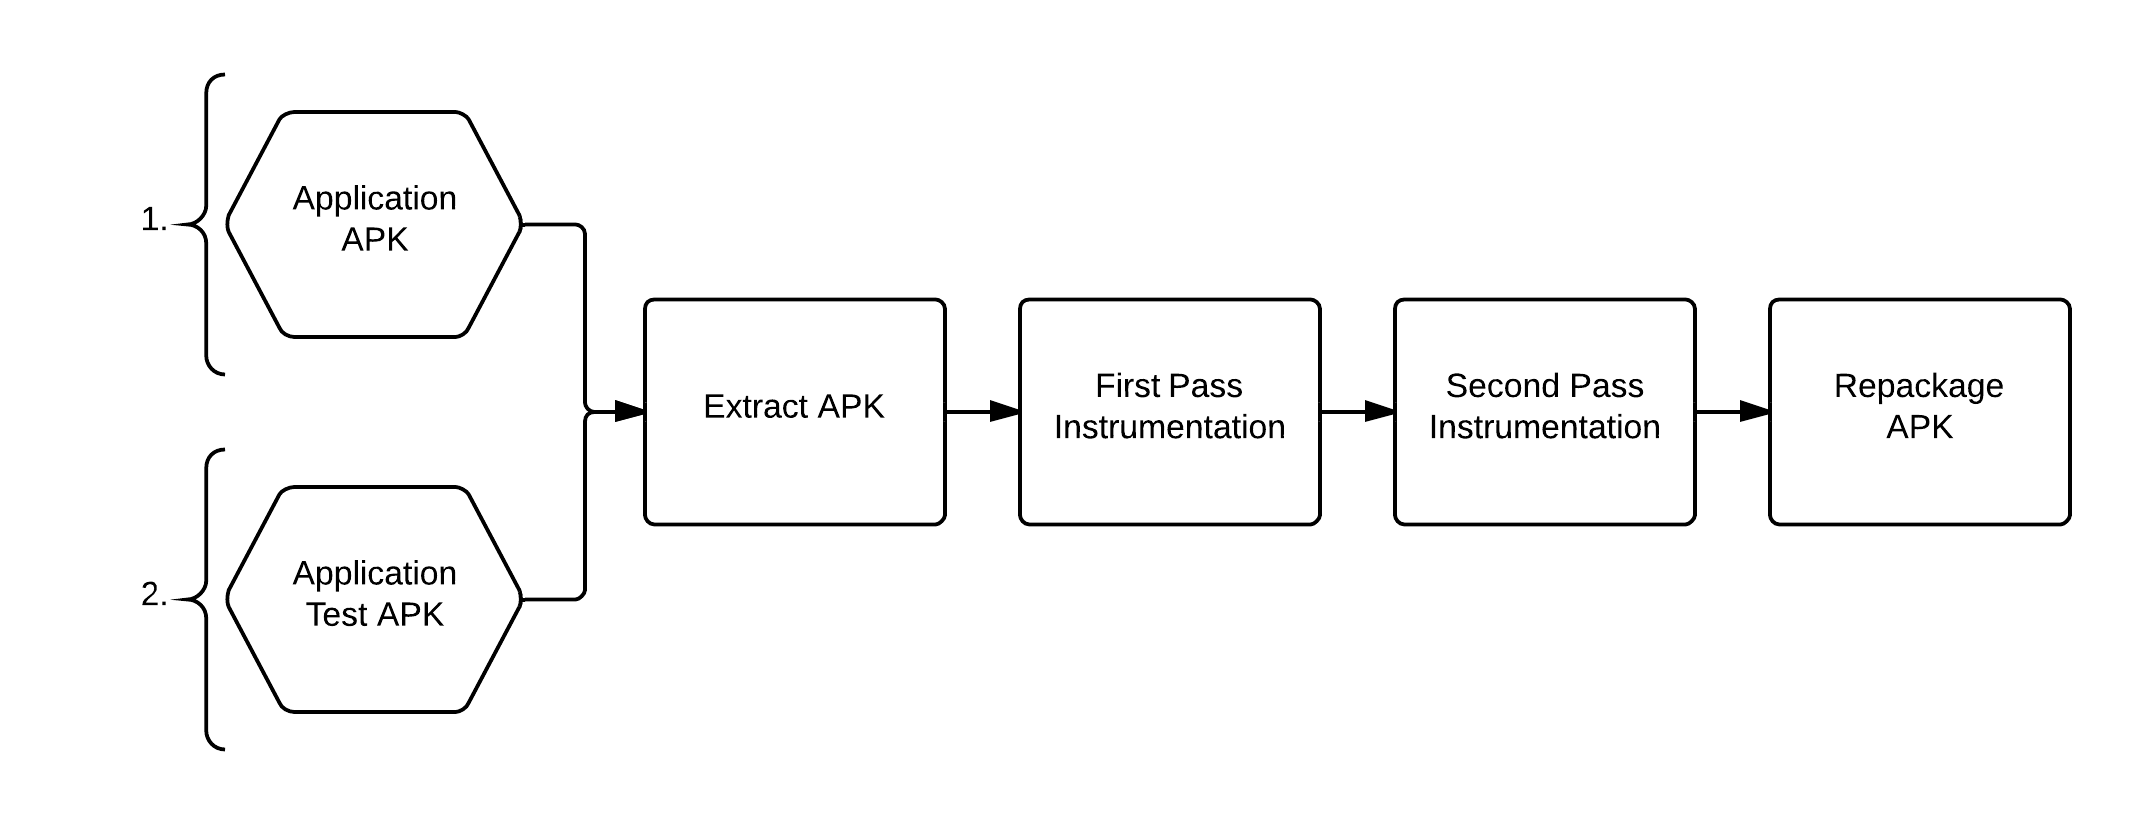
\includegraphics[width=\linewidth]{Images/instrumenting_apk}
\caption{}
\label{fig:instrumenting_apk}
\end{figure}

\subsubsection{Extraction}

\subsubsection{First Pass}

The first time, we build up a list of {\tt InstrumentationPoint} objects. These
correspond to the instrumentation points defined in \todo{sec:}. The proof of
concept supports method entry instrumentation points, and has basic
infrastructure for branch points, but no working support. At the moment, our
implementation is not adaptive --- instrumentation points are added
unconditionally provided they match a certain signature (\eg, method entry).
Each {\tt InstrumentationPoint} object has an associated {\tt
InstrumentationPolicy}. The tool assumes an {\tt InstrumentationPolicy} of {\tt
Complex} for now, unless a {\tt @Splatter} annotation is found with a different
policy. Section \todo{[]} defines the {\tt @Splatter} annotation and its
customizable parameters. Note that in the future, instrumentation points and the
like will be stored along with the test run results by the Jenkins plugin. Then,
the results will be given to this tool again, so that it can decide which
instrumentation policies to apply to each instrumentation point (\eg, an
instrumentation point with a previous {\tt InstrumentationPolicy} of {\tt
InstrumentationPolicy.COMPLEX} could be assigned a new policy of {\tt
InstrumentationPolicy.NONE} if the site has not been helpful in determining a
failure-predicting predicate and should not be monitored this time around).

\subsubsection{Second Pass}

Instrumentation bytecode is injected during the second pass. With a list of
instrumentation points defined, we visit the bytecode again, this time inserting
probes based on the {\tt InstrumentationPolicy} each time we encounter bytecode
that matches a known {\tt InstrumentationPoint}. As might be expected, a policy
of {\tt COMPLEX} tells us to inject a complex probe, {\tt SIMPLE} a simple
(counter-based) probe and {\tt NONE} nothing at all. Finally, at the end of the
second pass, any extra classes that we require for monitoring our
instrumentation are injected. \todo{Note that most of these classes are now
defined in the Splatter SDK?}.

The user must provide at least one base test class and the names of its
equivalent JUnit's {\tt SetUp} and {\tt TearDown} methods. These are methods
that are called respectively at the beginning and end of each individual test
run. We inject code to initialize and clean up our logging system at these
points. Upon {\tt SetUp}, we create a file matching the test name \todo{a
directory diagram with some tests} under the directory \todo{android
directories}.

\subsubsection{Injecting Instrumentation}

This section details the steps we take to insert probe at an instance method
entry and presents the results of both a complex and a simple probe in practice.

A Dalvik bytecode method consists of the definition and associated data. Most of
this data is of no consequence to our instrumentation, but we have to pay
attention to the registers.

Each method specifies the number of registers it requires. Arguments of a method
take the final registers, with the final argument taking the final register
position. Instance methods have a reference to their live object passed as the
first argument; the formal arguments (if any) take up the next registers in
order.

For the Java methods:

\begin{lstlisting}[mathescape, numberblanklines=false]
private String anExampleMethod(String firstArg, int secondArg) {
    return appendIntToString(firstArg, secondArg);
} (*@\SuppressNumber@*)
$\vdots$ (*@\ReactivateNumber@*)
private static String appendIntToString(String baseString, int number) {
    return baseString + number;
}
\end{lstlisting}

The corresponding Dalvik bytecode would be generated for {\tt anExampleMethod}:

\begin{lstlisting}[mathescape,numberblanklines=false]
#1              : (in Lcom/example/MainActivity;)
  name          : 'anExampleMethod'
  type          : '(Ljava/lang/String;I)Ljava/lang/String;'
  access        : 0x0002 (PRIVATE) (*@\SuppressNumber@*)
$\vdots$ (*@\ReactivateNumber@*)
  registers     : 4
  ins           : 3
  outs          : 2 (*@\SuppressNumber@*)
$\vdots$ (*@\ReactivateNumber@*)
024570:                  |[024570] com.example.MainActivity.anExampleMethod:(Ljava/lang/String;I)Ljava/lang/String; (*@\label{method_body_definition}@*)
024580: 7120 8503 3200   |0000: invoke-static {v2, v3}, Lcom/example/MainActivity;.appendIntToString:(Ljava/lang/String;I)Ljava/lang/String; // method@0385
024586: 0c00             |0003: move-result-object v0
024588: 1100             |0004: return-object v0 (*@\label{method_body_end_definition}@*) (*@\SuppressNumber@*)
$\vdots$ (*@\ReactivateNumber@*)
      locals    :
        0x0000 - 0x0005 reg=1 this Lcom/example/MainActivity;
        0x0000 - 0x0005 reg=2 firstArg Ljava/lang/String;
        0x0000 - 0x0005 reg=3 secondArg I
\end{lstlisting}

Lines \ref{method_body_definition}-\ref{method_body_end_definition} define the
method body. In this case, the method body simply returns void since it is empty
in the original Java source. The full set of bytecode operations and symbols are
defined at \cite{dalvikBytecode}. Note that this listing omits irrelevant
sections of bytecode. The full listing can be found in section
\ref{sec:sec:full_dalvik_bytecode_example}. From here on we will focus on the
registers, method body and locals of the bytecode, omitting extraneous
information as we see fit.

\todo{colour coded register allocation (Dalvik bytecode)}

\todo{Need to detail our register allocating visitor and explain how it works /
when it (might?) fail!}

\subsubsection{Storing the results}

With the tests running on the Android device or emulator, we must somehow
retrieve the {\tt JSON} logs either during the test run or afterward.
Transferring logs during the test run is unreliable. If we were to send our JSON
to {\tt logcat} with a special tag and monitor it on the build agent, we could
{\lq}miss{\rq} messages due to log flooding. Consider a heavily instrumented
application capable of logging a huge number of events in a short period of time
--- if data is written to the device's log buffer faster than {\tt logcat} can
read out of it, messages will be dropped. Instead, we log the {\tt JSON} to
files on the device's storage and retrieve it when the test suite has finished
running.

Copying the {\tt .json} log files back to the computer running the
instrumentation from the device with Gradle is a little tricky. Android provides
private storage for each installed application. It is possible, with root user
permissions, to access files in this space to manipulate them. However, as soon
as the tests finish executing, the Android Gradle plugin runs a private task
that uninstalls the application. When an application is removed, all of its
private data is deleted. Because the uninstall task is private, it is not
possible to hook in and run a simple shell script to retrieve the logs before
they are deleted.

We devised a workaround; Android has guaranteed {\lq}public{\rq} storage that is
not removed when an application is uninstalled. Its location is not fixed and is
likely to differ per-device and operating system version. So, we take care to
inform the build agent of the exact location of the devices public storage each
test run before copying the files.

When the tests finish running, we log a message with a special tag to {\tt
logcat} specifying the full path to the results directory on the device. Then, a
Gradle task grabs the {\tt logcat} logs, searches for the message and parses it
to get the location. Then, the task uses {\tt adb pull} and {\tt adb rm} to grab
and finally delete the files from the device. The previous issue of log flooding
can still be a problem here. If our special log message is lost in the noise of
an extreme number of log messages (i.e., deleted before we can grab it), the
build could fail. This is robust enough for a proof of concept.

\subsubsection{Soot}

We looked into Soot for its ability to generate control flow graphs (CFGs). When
searching for failure-predicting predicates, we will favor locations futher down
the CFG when placing probes (new or moved). Section \todo{ref} describes this
process in more detail.

It is possible to generate the CFG for a method using ASMDEX alone, although it
is a slightly more tricky task.

In the end, although Soot appeared to be a nice tool to work with, we scrapped
it for a few reasons. Firstly, the representation used by Soot is fairly
incompatible with that of ASMDEX. Even if we could determine the CFG for a
method using Soot, we'd have to somehow map the locations to our ASMDEX
instrumentation sites --- a non-trivial task. Finally, the overhead of starting
up Soot and loading an APK is significant. On an
Intel\textsuperscript{\textregistered} Core\textsuperscript{\texttrademark}
i7-3610QM CPU @ 2.30GHz, the the time to load the application and test APKs was
10.76 seconds. With a total instrumentation time of 19.09 seconds, Soot takes up
56\% of the total instrumentation time (and that is \textit{without} generating
the CFGs for any methods). In fact, with Soot removed entirely, the same
instrumentation run took just 3.294 seconds --- 17\% of the previous total run
time.

\subsubsection{Hardcoded Strings}

There are various points in the application that have been hardcoded during
development and never exposed to the user or calculated automatically. These are
marked with \texttt{// TODO:} comments in the places they do exist.

\subsection{Notes}

\subsubsection{SDK}

An SDK project can (optionally) be included. It defines the annotation
@SplatterIgnore. During the isntrumentation phase, if a method is found with
this annotation, it is blacklisted from the list of possible instrumentation
sites. This could be useful by developers during debugging, or to remove
instrumentation from sites that are known to be problematic or, alternatively,
{\lq}bug-free{\rq}!

\textbf{Methods} For methods that are not blacklisted or ignored due to
annotations, we store the method name and owner class (\todo{should also keep
track of signature / return type?}) in our pool of {\lq}method{\rq}
instrumentation points. During the second pass, these methods can be
instrumented with a complex (argument-saving) or simple (counter-based) probe IF
chosen during the WEKA stage.

\subsection{Logging to JSON}

\todo{Describe/show structure of log messages (show sample JSON for a method
call and the original Java code etc.). Perhaps also show the Dalvik bytecode?}

Logging runs on a background thread. The Test APK drives the Application APK.

\subsection{Analysis}

\todo{need to save the details of the probes we used and their associated
instrumentation points so that we can infer things!}

\subsection{Hooking into testrunners}

Part of our approach is to log distinct data per-test. To keep overhead to a
minimum, we take a map of test runner classes and their respective set up / tear
down methods (run before / after each test in a class is run). We inject our
logger set up and clean up to the setup / teardown methods respectively.

Note that during setup if the currently executing method has a @Splatter
annotation attached, we look at its policy before running the logging set up. If
the annotation has InstrumentationPolicy.NONE, we simply run the test as normal.

This means that within a class with multiple tests, we can disable
instrumentation on any subset of the tests if the developer so desires.

It is important to note that while the @Splatter annotation with an
instrumentation policy of NONE prevents the method itself from being
instrumented (and in the case of a test, also prevents the logging system from
being initialized), other methods will STILL potentially be instrumented. So a
test with the annotation and policy that initializes an Activity and performs a
sequence of actions will still have a performance penalty if called methods
happen to be instrumented.


\subsection{Modifying the Behaviour}

A small project ('splatter-sdk') can be included to force certain behaviour. It
is a simple library that defines a @Splatter annotation, with a parameter
{\lq}InstrumentationPolicy{\rq}. When a method is annoted with this and a policy
specified, Splatter will respect the defined behaviour when performing
instrumentation.

Available policies are:

\begin{itemize}
  \item NONE - Disallows all instrumentation from being injected in the method.
  When a test is given with this value, the logging system itself will not be
  initialized for that test.
  \item SIMPLE - Disallows complex probes from being injected in the containing
  method.
  \item COMPLEX - (Default), allows all probes to be potentially placed in the
  containing method.
\end{itemize}


\subsection{Logging Events}

Each event is created as a bean and held in a queue until it can be written to a
JSON output file. We define an abstract LogEvent bean with common values (System
Time, Thread, EventName etc.) and subclass for specific events.

\todo{We should log to a seperate blocking queue / file per thread since then we
won't get blocking occuring at runtime. We can then weave the seperate log files
together upon teardown.}


\subsection{A Solution}

\subsubsection{Identification}

After a test run completes, we can gather the test run artifacts (JUnit results,
\heisentest JSON log files \etc) and store them in a persistent database. In
the future, we can look at the test runs over time and attach various values to
each test much in the same way as the existing tools. \todo{Section [] describes
the values and things we expect to infer in more detail.}. TODO: Write a list of
values we hope to attach to each test. Back this up with quotes from Shazam.

\subsubsection{Prioritisation}

We can use the data gathered during the identification stage to rank the tests
according to criteria. A simple output would be a descending list ordered by
flakiness:

\begin{center}
    \begin{tabular}{ | l | p{5cm} |}
    \hline
    Test & Flakiness \% \\ \hline
    testVeryFlaky() & 91 \\ \hline
    testSometimesFlaky() & 33 \\ \hline
    testSignificantlyFlaky() & 2 \\ \hline
    \end{tabular}
\end{center}

Or, we could group the tests by common failure type, e.g.:

% \lstset{
% 	numbers=none,
% 	xleftmargin=3pt,
% 	numbersep=1em
% }

\begin{center}
    \begin{tabular}{| p{10cm} | l |}
    \hline
    Common Failure & \flaky Test Count \\ \hline
    {\begin{lstlisting}[language=Java, numbers=none]
java.lang.OutOfMemoryError
	\end{lstlisting}}
    & 4 \\ \hline
    {\begin{lstlisting}[language=Java, numbers=none]
java.lang.AssertionError:
Expected: (View visibility to be View.VISIBLE and View to have a width and a height)
but: View visibility to be View.VISIBLE View with id: class android.resources.R$id.anExampleView(1) had a visibility of View.GONE
	\end{lstlisting}}
	& 2 \\ \hline
    {\begin{lstlisting}[language=Java, numbers=none]
junit.framework.AssertionFailedError:
expected: "an_example_string"
but was: ""
	\end{lstlisting}}
	& 1 \\ \hline

    \end{tabular}
\end{center}

\flaky tests using the same troublesome method or similar logical flow may well
fail with the same stacktrace or assertion failure. By automatically detecting
this, developers could target groups of related tests and potentially fix an
entire group at once.

\subsubsection{Resolution}

Using data from the identification and prioritisation stages, we can begin to
develop an adaptive instrumentation to automatically gather runtime information
whilst maintaining a low overhead.

\todo{Explain why we are ‘just’ targeting Android for now (Shazam, GUI testing,
\etc).}

Automated testing is used during development. We therefore can assume
unrestricted access to debug builds.

\subsubsection{Future Work}

The plugin will need to analyse historical test results and calculate the
probability of failure for each test \todo{as discuss in section $n$}. It will
also need to be extended with an interface to visualise test flakiness and
related information {\todo bring in some of the information from approach here,
flakiness tables \etc}. This is also related to prioritisation.


\subsection{A Choice of Continuous Integration Tools}

Jenkins \cite{Jenkins} is a popular open source continuous integration tool.
Like others of its kind, it maintains a history of build results and their
associated artifacts. A wealth of plugins provide support for testing frameworks
such as JUnit --- displaying individual test outcomes, stack traces and
assertions in a simple interface.

Although there are many open source alternatives which we could support (\eg,
Hudson, from which the Jenkins project derives), many of these have
significantly smaller user bases and commit activity. Mostly though, our
decision to support Jenkins was motivated by Shazam's use of it across all
teams.

Although the tool will be developed initially for Jenkins, it is essential to
structure the plugin such that it can easily be migrated to other CI systems. At
all stages of design, this must be kept in mind.
